\chapter{NUMERICAL IMPLEMENTATION}

In this chapter, the mathematical details involved in the numerical solution of the previously described equations are presented.
It is assumed that this model is run in conjunction with a model describing the growth of kelp over its life cycle, which calls this light model periodically to update the light field.

\section{Kelp Numerics}

The algorithm described in this chapter has two components.
First, a probabilistic description of the kelp is generated at each point in a discrete spatial grid.
Second, optical properties of the resulting kelp-water medium are derived, and the light field is calculated.
The first component is described here.

\subsection{Length Distribution}

Rather than model each kelp frond, a subset of the population, called super-individuals, are modelled explicitly, and are considered to represent many identical individuals, as in \citep{scheffer_super-individuals_1994}.
Specifically, at each depth $k$, there are $n$ super-individuals, indexed by $i$.
Super-individual $i$ has a frond area $A_{ki}$ and represents $n_{ki}$ individual fronds.

From \eqref{eqn:length-from-area}, the frond length of the super-individual is $l_{ki} = \sqrt{2A_{ki}f_r}$.
Given the super-individual data, we calculate the mean $\mu$ and standard deviation $\sigma$ frond
lengths using the formulas:
\begin{equation}
  \mu_k = \frac{\ds \sum_{i=1}^N l_{ki}}{\ds \sum_{i=1}^N n_{ki}},
\end{equation}
\begin{equation}
  \sigma_k = \frac{\ds \sum_{i=1}^N \left( l_{ki} - \mu_k \right)^2}{\ds \sum_{i=1}^N n_{ki}}.
\end{equation}
We then assume that frond lengths are normally distributed in each depth layer
with mean $\mu_k$ and standard deviation $\sigma_k$.

\section{Discrete Grid}
The following is a description of the uniform, rectangular spatial-angular grid used
in the numerical implementation of this model.
It is assumed that all simulated quantities are constant over the interior of a
grid cell.

The number of grid cells in each dimension are denoted by $n_x$, $n_y$, $n_z$,
$n_\theta$, and $n_\phi$, with uniform spacings $dx$, $dy$, $dz$, $d\theta$, and
$d\phi$ between adjacent grid points.

The following indices are assigned to each dimension:
\begin{align}
  x &\to i \\
  y &\to j \\
  z &\to k \\
  \theta &\to l \\
  \phi &\to m
\end{align}

It is convenient, however, to use a single index $p$ to refer to directions $\vec{\omega}$ rather than referring to $\theta$ and $\phi$ separately.
Then, the center of a generic grid cell will be denoted as
$(x_i, y_j, z_k, \vec{\omega}_p)$, and the boundaries between adjacent grid cells
will be referred to as \textit{edges}.
One-indexing is employed throughout this document.

\subsection{Spatial Grid}
\begin{figure}[H]
  \centering
  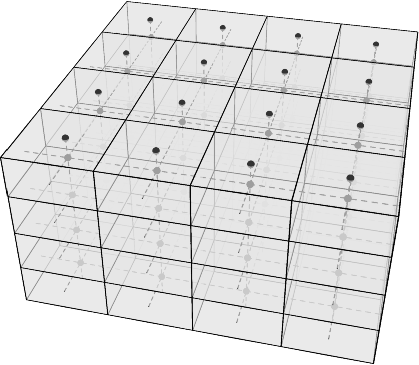
\includegraphics[width=8cm]{spatialgrid.pdf}
  \caption{Spatial grid}
  \label{fig:spatial_grid}
\end{figure}

\begin{align}
  dx &= \frac{x_{\max}-x_{\min}}{n_x} \\ 
  dy &= \frac{y_{\max}-y_{\min}}{n_y} \\ 
  dz &= \frac{z_{\max}-z_{\min}}{n_z}
\end{align}

Denote the edges as 
\begin{align}
  x_i^e &= (i-1)x \mbox{ for } i=1,\ldots,n_x \\
  y_j^e &= (j-1)y \mbox{ for } j=1,\ldots,n_y \\
  z_k^e &= (k-1)z \mbox{ for } k=1,\ldots,n_z 
\end{align}

and the cell centers as
\begin{align}
  x_i &= (i-1/2)dx \mbox{ for } i=1,\ldots,n_x \\
  y_j &= (j-1/2)dy \mbox{ for } j=1,\ldots,n_y \\
  z_k &= (k-1/2)dz \mbox{ for } k=1,\ldots,n_z
\end{align}

Note that in this convention, there are the same number of edges and cells,
and edges preceed centers.

% TODO: Not sure about this here.
Also, note that no grid center is located on the plane $z=0$.
The surface radiance boundary condition is treated separately.

\subsection{Angular Grid}
\begin{figure}[H]
  \centering
  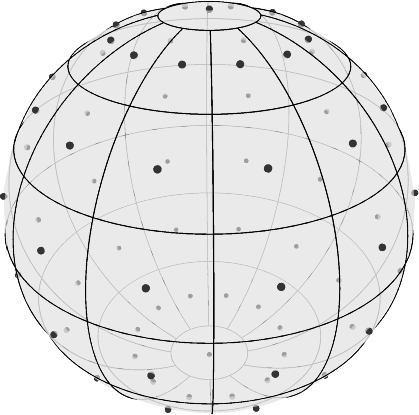
\includegraphics[width=8cm]{angulargrid.pdf}
  \caption{Angular grid}
  \label{fig:angular_grid}
\end{figure}

Now, we define the azimuthal angle such that
\begin{align}
  \theta_l = (l-1)d\theta.
\end{align}
For the sake of periodicity, we need
\begin{align}
  \theta_1 &= 0, \\
  \theta_{n_\theta} &= 2\pi-d\theta,
\end{align}
which requires
\begin{equation}
  d\theta = \frac{2\pi}{n_\theta}.
\end{equation}

For the polar angle, we similarly let
\begin{equation}
  \phi_m = (m-1)d\phi
\end{equation}

Since the polar azimuthal is not periodic, we also store the endpoint, so
\begin{align}
  \phi_1 &= 0, \\
  \phi_{n_\phi} &= \pi.
\end{align}

This gives us
\begin{align}
  d\phi &= \frac{\pi}{n_\phi-1}.
\end{align}

It is also useful to define the edges between angular grid cells as
\begin{alignat}{3}
  \theta_l^e &= (l-1/2) d\theta, &\quad l&=1,\ldots,n_\theta \\
  \phi_m^e &= (m-1/2) d\phi, &\quad m&=1,\ldots,n_\phi-1.
\end{alignat}

Note that while $\theta$ has its final edge following its final center, this is
not the case for $\phi$.

\begin{figure}[h]
  \centering
  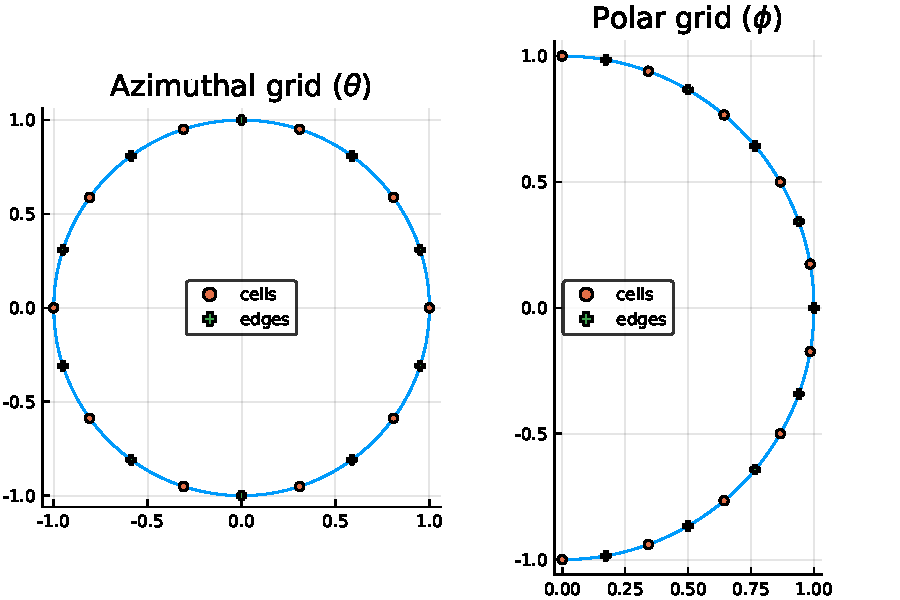
\includegraphics[width=.75\linewidth]{angular_grid_plots}
  \caption{Angular grid}
\end{figure}

As shown in Figure \ref{fig:angular_grid}, $\phi=0$ and $\phi=\pi$, called
the north ($+z$) and south ($-z$) poles respectively, are treated separately.
The total number of angles considered is $n_{\vec{\omega}} = n_\phi n_\theta -
2(n_\theta-1)$.
Since the poles create a non-rectangular angular grid in the sense that
$n_{\vec{\omega}}$ is not the product of two integers, it is advantageous to use
a single variable $p=1,\ldots,n_{\vec{\omega}}$ to index angles $\vec{\omega} =
(\theta, \phi)$ such that $p \in \left\{ 2,\ldots,n_{\vec{\omega}}-1 \right\}$ refers to the interior
of the angular grid, and $p=1$ and $p=n_{\vec{\omega}}$ refer to the
north and south poles respectively.
The following notation is used.
\begin{align}
  \hat{l}(p) &= \mbox{mod1}(p, n_\theta) \\
  \hat{m}(p) &= \ceil(p/n_\theta) + 1 \\
  \hat{\theta}_p &= \theta_{\hat{l}(p)} \\
  \hat{\phi}_p &= \phi_{\hat{m}(p)}
\end{align}

Thus, it follows that
\begin{equation}
  p = \left( \hat{m}(p)-2\right)n_\theta + \hat{l}(p).
\end{equation}

Accordingly, define
\begin{equation}
  \hat{p}(l,m) = (m-1)n_\theta + l.
\end{equation}

Further, we refer to the angular grid cell centered at $\vec{\omega}_p$ as $\Omega_p$, and the solid angle subtended by $\Omega_p$ is denoted $\abs{\Omega_p}$.
The areas of the grid cells are calculated as follows.
Note that there is a temporary abuse of notation in that the same symbols ($d\theta$ and $d\phi$) are being used for infinitessimal differential and for finite grid spacing.

For the poles, we have
\begin{align}
  \abs{\Omega_1} = \abs{\Omega_\nomega} &= \int_{\Omega_1} d{\vec{\omega}} \\
  &= \int_0^{2\pi}\int_0^{d\phi/2} \sin\phi\, d\phi\, d\theta \\
  &= 2\pi \cos\phi \Big|_{d\phi/2}^0 \\
  &= 2\pi(1-\cos(d\phi/2))
\end{align}

And for all other angular grid cells,
\begin{align}
  \abs{\Omega_p} &= \int_{\Omega_p} d{\vec{\omega}} \\
                 &= \int_{\theta_l^e}^{\theta_{l+1}^e}\int_{\phi_m^e}^{\phi_{m+1}^e} \sin(\phi)\, d\phi\, d\theta \\
                 &= d\theta \int_{\phi_m^e}^{\phi_{m+1}^e} \sin(\phi)\, d\phi \\
                 &= d\theta\left( \cos(\phi_m^e)-\cos(\phi_{m+1}^e) \right).
\end{align}


\subsection{Angular Quadrature}
We assume that all quantities are constant within a spatial-angular grid cell.
We therefore employ the midpoint rule for both spatial and angular integration.

Define the \textit{angular characteristic function}
\begin{equation}
  \mathcal{X}^\Omega_p(\vec{\omega}) = \begin{cases}
    1, & \vec{\omega} \in \Omega_p \\
    0, & \mbox{otherwise}
  \end{cases}
\end{equation}

\begin{align}
  \int_{4\pi} f(\vec{\omega})\, d\vec{\omega} &= \int_{4\pi} \sum_{p=1}^\nomega f_p \mathcal{X}^\Omega_p(\vec{\omega})\, d\vec{\omega} \\
  &= \sum_{p=1}^\nomega f_p \int_{4\pi} \mathcal{X}^\Omega_p(\vec{\omega})\, d\vec{\omega} \\
  &= \sum_{p=1}^\nomega f_p \int_{\Omega_p} d\vec{\omega} \\
  &= \sum_{p=1}^\nomega f_p \abs{\Omega_p}
\end{align}

 \subsection{Scattering Integral}

Specifically, we integrate $\beta$ to determine the amount of light scattered between angular grid cells.

Consider two angular grid cells, $\Omega$ and $\Omega'$.
The average probability density of scattering from $\vec{\omega} \in \Omega$ to $\vec{\omega}' \in \Omega'$ (or vice versa) is
\begin{equation}
  \beta_{pp'} = \frac{1}{\abs{\Omega}\abs{\Omega'}} \int_\Omega\int_{\Omega'}\beta(\vec{\omega}\cdot\vec{\omega}')\, d\vec{\omega'}\, d\vec{\omega}
\end{equation}

Denote the radiance at $(x_i, y_j, z_k, \vec{\omega}_p)$ by $L_{ijkp}$.
% TODO: Be more careful here.
Then, the total radiance scattered into $\Omega_p$ from $\Omega_{p'}$ is
\begin{align}
  \int_{\Omega}\int_{\Omega'}\beta(\vec{\omega} \cdot \vec{\omega}')L(\vec{x},\vec{\omega}')\, d\vec{\omega}'\, d\vec{\omega}
  &= L_{ijkp'} \int_\Omega\int_{\Omega_{p'}} \beta(\vec{\omega} \cdot \vec{\omega}')\, d\vec{\omega}'\, d\vec{\omega} \\
  &= \beta_{pp'}\abs{\Omega}\abs{\Omega'}L_{ijkp'}.
\end{align}
Hence, the average radiance scattered is $\beta_{pp'}\abs{\Omega'}L_{ijkp'}.$

\section{Finite Difference}

We now discuss the discretization of derivatives on the spatial grid.

\subsection{Discretization}

For the spatial interior of the domain, we use the 2nd order central difference formula (CD2) to approximate the derivatives, which is
\begin{equation}
    \tag{CD2}
    f'(x) = \frac{f(x+dx)-f(x-dx)}{2dx} + \mathcal{O}(dx^3).
\end{equation}

When applying the PDE on the upper or lower boundary, we use the forward and backward difference (FD2 and BD2) formulas respectively.
Omitting $\mathcal{O}(dx^3)$, we have
\begin{equation}
    \tag{FD2}
    \label{eq:FD2}
    f'(x) = \frac{-3f(x)+4f(x+dx)-f(x+2dx)}{2dx}
\end{equation}
\begin{equation}
    \tag{BD2}
    \label{eq:BD2}
    f'(x) = \frac{3f(x)-4f(x-dx)+f(x-2dx)}{2dx}
\end{equation}

For the upper and lower boundaries, we need an asymmetric finite difference
method.
In general, the Taylor Series of a function $f$ about $x$ is
\begin{equation}
  f'(x+\varepsilon) = \sum_{n=1}^\infty \frac{f^{(n)}(x)}{n!} \varepsilon^n \\
\end{equation}

Truncating after the first few terms, we have
\begin{equation}
  \label{eqn:afd1}
  f'(x+\varepsilon)  = f(x) + f'(x)\varepsilon + \frac{f''(x)}{2}\varepsilon^2 + \mathcal{O}(\varepsilon^3)
\end{equation}

Similarly, replacing $\varepsilon$ with $-\varepsilon/2$ we have
\begin{equation}
  \label{eqn:afd2}
  f'(x-\frac{\varepsilon}{2}) = f(x) - \frac{f'(x)\varepsilon}{2} + \frac{f''(x)\varepsilon^2}{8} + \mathcal{O}(\varepsilon^3).
\end{equation}

Rearranging \eqref{eqn:afd1} produces
\begin{equation}
  \label{eqn:afd3}
  f''(x)\varepsilon^2 = 2f(x+\varepsilon) - 2f(x) - 2f'(x)\varepsilon + \mathcal{O}(\varepsilon^3)
\end{equation}

Combining \eqref{eqn:afd2} with \eqref{eqn:afd3} gives
\begin{align*}
  \varepsilon f'(x) &= 2f(x) - 2f(x-\frac{\varepsilon}{2}) + f''(x)\frac{\varepsilon^2}{8} + \mathcal{O}(\varepsilon^3) \\
                    &= 2f(x) - 2f(x-\frac{\varepsilon}{2}) + \frac{f(x+\varepsilon)}{4} - \frac{f(x)}{4} - \frac{f'(x)\varepsilon}{4} + \mathcal{O}(\varepsilon^3) \\
                    &= \frac{4}{5}\left( 2f(x)-2f(x-\frac{\varepsilon}{2}) + \frac{f(x+\varepsilon)}{4} - \frac{f(x)}{4} \right) + \mathcal{O}(\varepsilon^3)
\end{align*}

Then, dividing by $\varepsilon$ gives
\begin{equation}
  f'(x) = \frac{-8f(x-\frac{\varepsilon}{2}) + 7f(x) + f(x+\varepsilon)}{5\varepsilon} + \mathcal{O}(\varepsilon^2)
\end{equation}

Similarly, substituting $\varepsilon \to -\varepsilon$, we have 
\begin{equation}
  f'(x) = \frac{- f(x-\varepsilon) - 7f(x) + 8f(x+\frac{\varepsilon}{2})}{5\varepsilon} + \mathcal{O}(\varepsilon^2)
\end{equation}


\subsection{Difference Equation}

%TODO: Periodic $x,y$

In general, we have

\begin{equation}
  \vec{\omega} \cdot \nabla L_p = -(a+b) L_p + \sum_{p'=1}^{n_{\vec{\omega}}} \beta_{pp'}L_{p'}.
\end{equation}

Then,
\begin{equation}
  \vec{\omega} \cdot \nabla L_p + (a+b(1-\beta_{pp'}))L_p - \sum_{p'=1}^{n_{\vec{\omega}}} \beta_{pp'} L_{p'} = 0
\end{equation}

Interior:
\begin{equation}
  \begin{aligned}
    0 &= \frac{L_{i+1,jkp}-L_{i-1,jkp}}{2dx}\sin\hat{\phi}_p\cos\hat{\theta}_p \\
    &+ \frac{L_{i,j+1,kp}-L_{i,j-1,kp}}{2dy}\sin\hat{\phi}_p\sin\hat{\theta}_p \\
    &+ \frac{L_{ij,k+1,p}-L_{ij,k-1,p}}{2dz}\cos\hat{\phi}_p \\
    &+ (a_{ijk}+b(1-\beta_{pp'}))L_{ijkp}  - \sum_{p'=1}^{n_{\vec{\omega}}} \beta_{pp'} L_{ijkp'}
  \end{aligned}
\end{equation}

Surface downwelling (BC):
\begin{equation*}
  \begin{aligned}
    0 &= \frac{L_{i+1,jkp}-L_{i-1,jkp}}{2dx}\sin\hat{\phi}_p\cos\hat{\theta}_p \\
    &+ \frac{L_{i,j+1,kp}-L_{i,j-1,kp}}{2dy}\sin\hat{\phi}_p\sin\hat{\theta}_p \\
    &+ \frac{-8f_p + 7L_{ijkp} + L_{ij,k+1,p}}{5dz}\cos\hat{\phi}_p \\
    &+ (a_{ijk}+b(1-\beta_{pp'}))L_{ijkp} \\
    &- \sum_{p'=1}^{n_{\vec{\omega}}} \beta_{pp'} L_{ijkp'}.
  \end{aligned}
\end{equation*}

Combining $L_{ijkp}$ terms on the left and moving the boundary condition to the
right gives

\begin{equation}
  \begin{aligned}
    &\frac{L_{i+1,jkp}-L_{i-1,jkp}}{2dx}\sin\hat{\phi}_p\cos\hat{\theta}_p \\
    + &\frac{L_{i,j+1,kp}-L_{i,j-1,kp}}{2dy}\sin\hat{\phi}_p\sin\hat{\theta}_p \\
    + &\frac{L_{ij,k+1,p}}{5dz}\cos\hat{\phi}_p \\
    + &(a_{ijk}+b(1-\beta_{pp'}) + \frac{7}{5dz} \cos\hat{\phi}_p)L_{ijkp} \\
    - &\sum_{p'=1}^{n_{\vec{\omega}}} \beta_{pp'} L_{ijkp'} = \frac{8f_p}{5dz} \cos\hat{\phi}_p.
  \end{aligned}
\end{equation}

Likewise for the bottom boundary condition, we have

\begin{equation}
  \begin{aligned}
    0 &= \frac{L_{i+1,jkp}-L_{i-1,jkp}}{2dx}\sin\hat{\phi}_p\cos\hat{\theta}_p \\
    &+ \frac{L_{i,j+1,kp}-L_{i,j-1,kp}}{2dy}\sin\hat{\phi}_p\sin\hat{\theta}_p \\
    &- \frac{L_{ij,k-1,p}}{5dz}\cos\hat{\phi}_p \\
    &+ (a_{ijk}+b(1-\beta_{pp'}) - \frac{7}{5dz}\cos\hat{\phi}_p)L_{ijkp} \\
    &- \sum_{p'=1}^{n_{\vec{\omega}}} \beta_{pp'} L_{ijkp'}.
  \end{aligned}
\end{equation}

Now, for upwelling light at the first depth layer (non-BC), we apply FD2.
\begin{equation}
  \begin{aligned}
    0 &= \frac{L_{i+1,jkp}-L_{i-1,jkp}}{2dx}\sin\hat{\phi}_p\cos\hat{\theta}_p \\
    &+ \frac{L_{i,j+1,kp}-L_{i,j-1,kp}}{2dy}\sin\hat{\phi}_p\sin\hat{\theta}_p \\
    &+ \frac{-3L_{ijkp} + 4L_{ij,k+1,p} - L_{ij,k+2,p}}{2dz}\cos\hat{\phi}_p \\
    &+ (a_{ijk}+b(1-\beta_{pp'}))L_{ijkp} \\
    &- \sum_{p'=1}^{n_{\vec{\omega}}} \beta_{pp'} L_{ijkp'}.
  \end{aligned}
\end{equation}

Grouping $L_{ijkp}$ terms gives
\begin{equation}
  \begin{aligned}
    0 &= \frac{L_{i+1,jkp}-L_{i-1,jkp}}{2dx}\sin\hat{\phi}_p\cos\hat{\theta}_p \\
    &+ \frac{L_{i,j+1,kp}-L_{i,j-1,kp}}{2dy}\sin\hat{\phi}_p\sin\hat{\theta}_p \\
    &+ \frac{4L_{ij,k+1,p} - L_{ij,k+2,p}}{2dz}\cos\hat{\phi}_p \\
    &+ \left(a_{ijk}+b(1-\beta_{pp'}) - 3\frac{\cos\hat\phi_p}{2dz} \right)L_{ijkp} \\
    &- \sum_{p'=1}^{n_{\vec{\omega}}} \beta_{pp'} L_{ijkp'}.
  \end{aligned}
\end{equation}

Similarly, for downwelling light at the lowest depth layer, we have
\begin{equation}
  \begin{aligned}
    0 &= \frac{L_{i+1,jkp}-L_{i-1,jkp}}{2dx}\sin\hat{\phi}_p\cos\hat{\theta}_p \\
    &+ \frac{L_{i,j+1,kp}-L_{i,j-1,kp}}{2dy}\sin\hat{\phi}_p\sin\hat{\theta}_p \\
    &+ \frac{-4L_{ij,k-1,p} + L_{ij,k-2,p}}{2dz}\cos\hat{\phi}_p \\
    &+ \left(a_{ijk}+b(1-\beta_{pp'}) + 3\frac{\cos\hat\phi_p}{2dz} \right)L_{ijkp} \\
    &- \sum_{p'=1}^{n_{\vec{\omega}}} \beta_{pp'} L_{ijkp'}
  \end{aligned}
\end{equation}

\subsection{Structure of Linear System}

%TODO: This
Describe layout of matrix.

\begin{table}[H]
  \centering
  \begin{tabular}{p{\linewidth/3}p{\linewidth/3}p{\linewidth/3}}
    \toprule
    \textbf{Derivative case} & \textbf{\# nonzero/row} & \textbf{\# of rows} \\
    \midrule
    interior & $\nomega+6$ & $n_xn_y(n_z-2)\nomega$ \\
    surface downwelling & $\nomega+5$ & $n_xn_y\nomega/2$ \\
    bottom upwelling & $\nomega+5$ & $n_xn_y\nomega/2$ \\
    surface upwelling & $\nomega+6$ & $n_xn_y\nomega/2$ \\
    bottom downwelling & $\nomega+6$ & $n_xn_y\nomega/2$ \\
  \end{tabular}
  \caption{Breakdown of nonzero matrix elements by derivative case}
\end{table}

Number of rows/columns: $n_xn_yn_zn_{\vec{\omega}}$

Number of nonzero RHS entries: $n_xn_yn_z/2$

Total number of nonzero matrix entries: $n_xn_yn_{\vec{\omega}} \left[n_z(n_{\vec{\omega}}+6)-1 \right]$

\section{GMRES}
% TODO: Fill this in
GMRES is a Krylov Subspace method. These work like this. Here's what's special
about GMRES. Advantages. Drawbacks. Not practical for running in SINMOD.

\section{Numerical Asymptotics}

\subsection{Ray Tracing Algorithm}
% TODO: Revise
\subsubsection{Extract values along path}

In order to evaluate a path integral through the previously described grid, it
is first necessary to construct a one-dimensional piecewise constant integrand
which is discontinuous at unevenly spaced points corresponding to the
intersections between the path and edges in the spatial grid.

Consider a grid center $\vec{p_1} = (p_{1x},p_{1y},p_{1z})$ and a corresponding path $\vec{l}(\vec{x_1}, \vec{\omega}, s)$.
To find the location of discontinuities in the itegrand, we first calculate the
distance from its origin, $\vec{p_0} = \vec{x_0}(\vec{p_1}, \vec{\omega}) = (p_{0x}, p_{0y}, p_{0z})$ to grid edges in each dimension
separately.

Given
\begin{align}
  x_i &= p_{0x} + \frac{s_i^x}{\tilde{s}}(p_{1x}-p_{0x}) \\
  y_j &= p_{0y} + \frac{s_j^y}{\tilde{s}}(p_{1y}-p_{0y}) \\
  z_k &= p_{0z} + \frac{s_k^z}{\tilde{s}}(p_{1z}-p_{0z})
\end{align}

we have
\begin{align}
  s_i^x &= \tilde{s}\frac{x_i-p_{0x}}{p_{1x}-p_{0x}} \\
  s_i^y &= \tilde{s}\frac{y_i-p_{0y}}{p_{1y}-p_{0y}} \\
  s_i^z &= \tilde{s}\frac{z_i-p_{0z}}{p_{1z}-p_{0z}} \\
\end{align}


We also keep a record for each dimension specifying whether the ray increases
or decreases in the dimension. Let
\begin{align}
  \delta_x &= \sign(p_{0x}-p_{1x}) \\
  \delta_y &= \sign(p_{0y}-p_{1y}) \\
  \delta_z &= \sign(p_{0z}-p_{1z})
\end{align}

For convenience, we also store a closely related quantity, $\sigma$ with a value 1 for
increasing rays and 0 for decreasing rays in each dimension
\begin{align}
  \sigma_x = (\delta_x+1)/2 \\
  \sigma_y = (\delta_y+1)/2 \\
  \sigma_z = (\delta_z+1)/2
\end{align}

For this algorithm, we keep two sets of indices. $(i,j,k)$ indexes the grid
cell, and will be used for extracting physical quantities from each cell along
the path.
Meanwhile, $(i^e,j^e,k^e)$ will index the edges between grid cells, beginning
after the first cell. i.e., $i^e=1$ refers not to the plane $x=\xmin$, but to $x=\xmin+dx$.

Let $(i_0, j_0, k_0)$ be the indices of the grid cell containing $\vec{p_0}$.

That is,

\begin{align}
  i_0 &= \ceil\left(\frac{p_{0x}-\xmin}{dx}\right) \\
  j_0 &= \ceil\left(\frac{p_{0y}-\ymin}{dy}\right) \\
  k_0 &= \ceil\left(\frac{p_{0z}-\zmin}{dz}\right)
\end{align}

Then,
\begin{align}
  i_0^e &= i_0 + \sigma_x \\
  j_0^e &= j_0 + \sigma_y \\
  k_0^e &= k_0 + \sigma_z
\end{align}

Now, we calculate the distance from $p_0$ along the path to edges in each dimension.
\begin{align}
  s_i^x = \hat{s}\frac{x_i^e-p_{0x}}{p_{1x}-p_{0x}} \\
  s_j^y = \hat{s}\frac{y_j^e-p_{0y}}{p_{1y}-p_{0y}} \\
  s_k^z = \hat{s}\frac{z_k^e-p_{0z}}{p_{1z}-p_{0z}}
\end{align}

For each grid cell, we check the path lengths required to cross an $x$, $y$, and
$z$ edge-planes.
Then, we move to the next grid cell in that dimension.
That is,

% TODO: Check
* We also track $s$, the path length.

Consider $i,j,k$ fixed (denoting the current grid cell).

\begin{align}  
  d = \mbox{argmin}_{x,y,z} \left\{ s_i^x-s, s_j^y-s, s_k^z \right\}
\end{align}

Then,
% TODO: Fix this
* This doesn't quite make sense yet.
\begin{align}
  \begin{cases}
    i = i+\delta_x, & \mbox{if } d=x \\
    j = j+\delta_y, & \mbox{if } d=y \\
    z = k+\delta_z, & \mbox{if } d=z
  \end{cases}
\end{align}

and

\begin{align}
  \begin{cases}
    i^e = i^e+\delta_x, & \mbox{if } d=x \\
    j^e = j^e+\delta_y, & \mbox{if } d=y \\
    z^e = k^e+\delta_z, & \mbox{if } d=z
  \end{cases}
\end{align}


Then, move to the adjacent grid cell in the dimension which requires the shortest
step to reach an edge. Save $ds$ of the path through this cell. Also save abs.
coef. and source.
% TODO: Improve
** Definitely needs more work**

- absorption coefficient ($\tilde{a}(s)$)

- effective source ($g_n(s)$)

\subsubsection{Ray integral}

Here are the equations for calculating the double integral over ray paths
required for the asymptotics. It will hopefully make more sense once I add words
to accompany the symbols.

Let
\begin{align}
  g_n(s) &= \sum_{i=1}^{N-1}g_{ni}\mathcal{X}_i(s) \\
  \tilde{a}(s) &= \sum_{i=1}^{N-1}\tilde{a}_{i}\mathcal{X}_i(s) \\
\end{align}

and
\begin{equation}
  \mathcal{X}_i(s) = \begin{cases}
    1, & a_I \leq s < s_{i+1} \\
    0, & \mbox{otherwise}
    \end{cases}
\end{equation}

and $\left\{s_i\right\}_{i=1}^N$ is increasing.

Let $ds_i = s_{i+1} - s_i$.

Let $\hat{i}(s) = \min\left\{ i \in \{1,\ldots,N\} : s_i>s \right\}$.
Let $\tilde{d}(s) = s_{\hat{i}(s)}-s$.

We have $s_1 = 0$ and $s_N = \tilde{s}$.


\begin{align}
  u_n(\tilde{s}) &= \int_0^{\tilde{s}}g_n(s')\exp\left( -\int_{s''}^{s'}\tilde{a}(s'')\,ds'' \right)\, ds' \\
  &= \int_0^{s_N} \sum_{i=1}^{N-1}g_{ni}\mathcal{X}_i(s') \exp\left( -\int_{s''}^{s'}\sum_{j=1}^{N-1}\tilde{a}_{j}\mathcal{X}_j(s'')\,ds'' \right)\, ds' \\
  &= \sum_{i=1}^{N-1}g_{ni}\int_0^{s_N} \mathcal{X}_i(s') \exp\left( -\sum_{j=1}^{N-1}\tilde{a}_{j}\int_{s''}^{s'}\mathcal{X}_j(s'')\,ds'' \right)\, ds' \\
  &= \sum_{i=1}^{N-1}g_{ni}\int_{s_i}^{s_{i+1}}  \exp\left(-\tilde{a}_{\hat{i}(s')-1}\tilde{d}(s') -\sum_{j=\hat{i}(s')}^{N-1}\tilde{a}_{j}ds_j\right)\, ds' \\
  &= \sum_{i=1}^{N-1}g_{ni}\int_{s_i}^{s_{i+1}}  \exp\left(-\tilde{a}_{i}(s_{i+1}-s') -\sum_{j=i+1}^{N-1}\tilde{a}_{j}ds_j\right)\, ds'
\end{align}

Let
\begin{equation}
  b_i = -\tilde{a}_{i}s_{i+1} - \sum_{j=i+1}^{N-1}\tilde{a}_{j}ds_j.
\end{equation}

Then,
\begin{align}
  u_n(\tilde{s}) &= \sum_{i=1}^{N-1}g_{ni}\int_{s_i}^{s_{i+1}}  \exp\left(\tilde{a}_{i}s' + b_i\right)\, ds' \\
                 &= \sum_{i=1}^{N-1}g_{ni}e^{b_i}\int_{s_i}^{s_{i+1}}  \exp\left(\tilde{a}_{i}s'\right) ds'
\end{align}

Let
\begin{align}
  d_i &= \int_{s_i}^{s_{i+1}}  \exp\left(\tilde{a}_{i}s'\right)\, ds' \\
    &= \begin{cases}
    ds_i, & \tilde{a} = 0 \\
      \left( \exp(\tilde{a}_i s_{i+1}) - \exp(\tilde{a}_i s_i) \right)/\tilde{a}_i, & \mbox{otherwise}
    \end{cases}
\end{align}

Then,
\begin{equation}
  u_n(\tilde{s}) = \sum_{i=1}^{N-1} g_{ni}d_i e^{b_i}
\end{equation}
